\documentclass[12pt]{article}
%%%%%%%%%%%%%%%%
% Packages
%%%%%%%%%%%%%%%%

\usepackage[top=1cm,bottom=1.25cm,left=1.25cm,right= 1.25cm]{geometry}
\usepackage[parfill]{parskip}
\usepackage{graphicx, fontspec, xcolor,multicol, enumitem, setspace, amsmath, changepage}
\DeclareGraphicsRule{.tif}{png}{.png}{`convert #1 `dirname #1`/`basename #1 .tif`.png}

%%%%%%%%%%%%%%%%
% User defined colors
%%%%%%%%%%%%%%%%

% Pantone 2015 Fall colors
% http://iwork3.us/2015/02/18/pantone-2015-fall-fashion-report/
% update each semester or year

\xdefinecolor{custom_blue}{rgb}{0, 0.32, 0.48} % FROM SPRING 2016 COLOR PREVIEW
\xdefinecolor{custom_darkBlue}{rgb}{0.20, 0.20, 0.39} % Reflecting Pond  
\xdefinecolor{custom_orange}{rgb}{0.96, 0.57, 0.42} % Cadmium Orange
\xdefinecolor{custom_green}{rgb}{0, 0.47, 0.52} % Biscay Bay
\xdefinecolor{custom_red}{rgb}{0.58, 0.32, 0.32} % Marsala

\xdefinecolor{custom_lightGray}{rgb}{0.78, 0.80, 0.80} % Glacier Gray
\xdefinecolor{custom_darkGray}{rgb}{0.35, 0.39, 0.43} % Stormy Weather

%%%%%%%%%%%%%%%%
% Color text commands
%%%%%%%%%%%%%%%%

%orange
\newcommand{\orange}[1]{\textit{\textcolor{custom_orange}{#1}}}

% yellow
\newcommand{\yellow}[1]{\textit{\textcolor{yellow}{#1}}}

% blue
\newcommand{\blue}[1]{\textit{\textcolor{blue}{#1}}}

% green
\newcommand{\green}[1]{\textit{\textcolor{custom_green}{#1}}}

% red
\newcommand{\red}[1]{\textit{\textcolor{custom_red}{#1}}}

%%%%%%%%%%%%%%%%
% Coloring titles, links, etc.
%%%%%%%%%%%%%%%%

\usepackage{titlesec}
\titleformat{\section}
{\color{custom_blue}\normalfont\Large\bfseries}
{\color{custom_blue}\thesection}{1em}{}
\titleformat{\subsection}
{\color{custom_blue}\normalfont}
{\color{custom_blue}\thesubsection}{1em}{}

\newcommand{\ttl}[1]{ \textsc{{\LARGE \textbf{{\color{custom_blue} #1} } }}}

\newcommand{\tl}[1]{ \textsc{{\large \textbf{{\color{custom_blue} #1} } }}}

\usepackage[colorlinks=false,pdfborder={0 0 0},urlcolor= custom_orange,colorlinks=true,linkcolor= custom_orange, citecolor= custom_orange,backref=true]{hyperref}

%%%%%%%%%%%%%%%%
% Instructions box
%%%%%%%%%%%%%%%%

\newcommand{\inst}[1]{
\colorbox{custom_blue!20!white!50}{\parbox{\textwidth}{
	\vskip10pt
	\leftskip10pt \rightskip10pt
	#1
	\vskip10pt
}}
\vskip10pt
}

%%%%%%%%%%%
% App Ex number    %
%%%%%%%%%%%

% DON'T FORGET TO UPDATE

\newcommand{\appno}[1]
{1}

%%%%%%%%%%%%%%
% Turn on/off solutions       %
%%%%%%%%%%%%%%

% Off
\newcommand{\soln}[2]{$\:$\\ \vspace{#1}}{}

%% On
%\newcommand{\soln}[2]{\textit{\textcolor{custom_red}{#2}}}{}

%%%%%%%%%%%%%%%%
% Document
%%%%%%%%%%%%%%%%

\begin{document}
\fontspec[Ligatures=TeX]{Helvetica Neue Light}

Dr. \c{C}etinkaya-Rundel \hfill Sta 101: Data Analysis and Statistical Inference \\
Duke University - Department of Statistical Science \hfill \\

\ttl{Discussion section \appno{}: Math review}

$\:$ \\

\begin{enumerate}

\item Which of the following is the smallest?

\begin{enumerate}
\item $3/4$
\item $4/5$
\item $59/60$
\item $100/101$ \\
\end{enumerate}

\item If $3x - x + 6x = 5y - 20$, and if $y = 8$, what is the value of $x$? \\

\item You are given the following equation:

\[ a = 1.96 \sqrt{\frac{p (1-p)}{n}} \]

You are also told that:

\begin{itemize}
\item $p = 0.3$
\item $a$ cannot be larger than 0.06
\item $n$ is a whole number
\end{itemize}

What is the lowest value $n$ can take on? \\

\item Two jars, A and B, are filled with pink and blue chips. Jar A has 6 pink and 60 blue chips. Jar B has 4 pink and 40 blue chips. You shake both jars and draw a chip from each without looking. Which container gives you the best chance of drawing a pink marble? \\

\item There are 10 cats in a shelter. Mine wants to adopt at most 3 cats. What are the possible number of cats she can adopt? \\

\item On a game show, 10 questions are asked to contestants. If a contestant gets at least one question wrong, they lose the entire game. How many questions should contestants get right to win the game? \\

\pagebreak

\item In the Venn diagrams below, shade the following areas:

\begin{multicols}{2}
\begin{enumerate}
\item A but not B

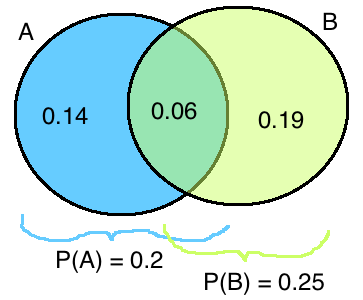
\includegraphics[width=0.3\textwidth]{venn.gif}

\item A and B

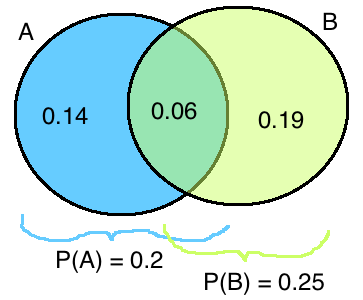
\includegraphics[width=0.3\textwidth]{venn.gif}

\item A or B

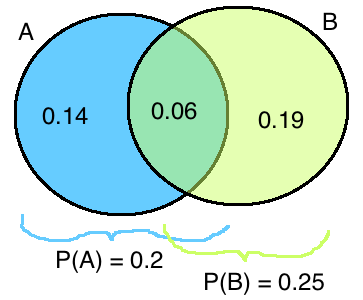
\includegraphics[width=0.3\textwidth]{venn.gif}

\item neither A nor B

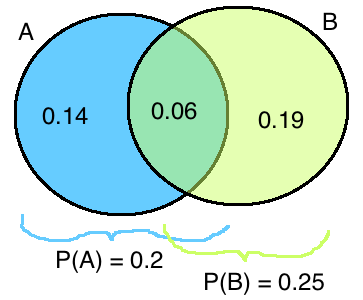
\includegraphics[width=0.3\textwidth]{venn.gif}

\end{enumerate}
\end{multicols}

\item Solve $3 (6 + 4) (5 - 3)$. \\

\item The standard deviation is defined as

\[ s = \sqrt{ \frac{\sum_{i = 1}^n (x_i - \bar{x})^2}{n - 1} } \]

What is the standard deviation of the following dataset: \{5, 8, 5, 4, 8\}? \\

\item Which of the following datasets has a higher standard deviation? Answer without actually calculating the standard deviation.

\begin{enumerate}
\item 3, 4, 5, 5, 6
\item 100, 100, 100, 100, 101
\end{enumerate}

\end{enumerate}

\end{document}